\documentclass[11pt]{article}

\usepackage[margin=1in]{geometry}
\usepackage{graphicx}
\usepackage{amsmath,amssymb}
\usepackage{booktabs}
\usepackage{float}
\usepackage[colorlinks=true,linkcolor=blue,citecolor=blue,urlcolor=blue]{hyperref}
\usepackage{caption}
\usepackage{siunitx}

\title{On the Inaccuracy of Global Optimization Methods\\ to Extract ReRAM Parameters}
\author{
  R.~Picos \and C.~de Benito \and O.~Camps \\[0.3em]
  \small Industrial Engineering and Construction Department, Universitat de les Illes Balears, Spain
}
\date{}

\begin{document}
\maketitle

\begin{abstract}
We fit the Dynamic Memdiode Model (DMM) of Miranda et al.\ to a 14\,604-cycle
HfO$_2$ ReRAM switching-current dataset, using five distinct parameter-extraction
strategies: gradient-based least squares, a genetic algorithm, a directed
genetic algorithm steered by the local Jacobian's principal directions, a
genetic-algorithm/least-squares hybrid, and a neural-network surrogate trained
on realistic synthetic data. All five reproduce the measured current to within
a few percent. None of them reliably recovers the underlying twelve model
parameters. We show this with a Monte Carlo test against a known, noise-free
synthetic ground truth: even there, several parameters -- most persistently
the SET threshold voltage $v_s$, the SET nonlinearity pair $(a_{on}, i_{on})$,
and the RESET rate constant $\eta_r$ -- are recovered with correlations to
truth no better than 0.1--0.3, regardless of optimizer. We trace this to a
structural, not algorithmic, cause: every cycle in the dataset is excited by
the same fixed voltage waveform, which does not carry enough independent
information to pin down every parameter of a twelve-parameter nonlinear ODE.
We corroborate this directly with a new test reported here: pooling
$a_{on}, i_{on}$ as shared constants across twelve real measurement windows,
instead of fitting them per window, multiplies the fit error by a factor of
14.6 uniformly across every window, ruling out the simplest fix one would
try. A sixth, categorically different method -- a non-gradient, rule-based
extractor with no joint cost function at all -- fails the same benchmark
even more starkly: five of its ten free parameters never move from their
initial seed across the entire 250-cycle run, which we read as further,
optimizer-independent evidence for the same conclusion. We also describe
the subset of extraction relations that \emph{can} be
derived directly from the model's own equations and validated exactly, the
production fitting procedure used to generate the dataset-wide results, and
release the parameter-trajectory viewer used throughout this work as a public
tool.
\end{abstract}

\section{Introduction}

Compact modeling of resistive switching devices has mostly been judged by
how well a model reproduces the major $I$-$V$ hysteresis loop. This is a weak
test: a model with more free parameters than the data can constrain will
often match the loop closely while assigning those parameters values that
have little to do with the device's actual physics. Hysteron behavior --
partial, minor loops traced out under sub-saturating excitation -- has
recently been proposed as a more stringent benchmark, since it probes the
device away from its two extreme states and is harder to fit by accident
\cite{miranda2026hysteron}. The Dynamic Memdiode Model (DMM) we use in this
work is one such model, and it is the one against which this paper's
findings are demonstrated; but the problem we describe is not specific to
it. It belongs to parameter extraction for resistive-switching compact
models generally, and shows up, in one form or another, in essentially
every model we could find in the literature that documents how its
parameters are actually obtained from data.

The Stanford/ASU RRAM model \cite{jiang2016compact} is calibrated against
experimental $I$-$V$ sweeps by nonlinear optimization, with cycle-to-cycle
variation captured afterwards as a distribution over the fitted parameters
rather than derived from first principles. The Simmons tunnel-barrier model
of Pickett et al.\ \cite{pickett2009switching}, one of the earliest
physically motivated switching-dynamics models, has several constants that
later authors describe plainly as fitting parameters without direct physical
meaning, extracted by matching switching data rather than read off a curve.
The TEAM/VTEAM family \cite{kvatinsky2015vteam} was designed with
extraction in mind -- its threshold voltages are meant to correspond to
visible features of the $I$-$V$ curve -- but even there the full parameter
set is obtained by numerical fitting, not a closed-form procedure. A 2025
preprint by Hamid and Hassan \cite{hamid2025cnn} tackles the Stanford and
VTEAM models with almost exactly the architecture we independently arrived
at for the DMM below: a convolutional network trained on synthetic data
produces an initial guess, refined afterwards by heuristic optimization.
Their own results report several parameters saturating at the imposed bounds
of the search space during fitting -- the same symptom, on a different
model, that we document in Section~\ref{sec:difficulty} for the DMM's
$a_{on}$. One genuinely different approach is the data-driven Verilog-A
model of Messaris et al.\ \cite{messaris2018datadriven}, which pairs the
model with dedicated characterization hardware that applies a chosen
sequence of pulses to the physical device and extracts parameters from the
elicited response; this sidesteps the identifiability problem by controlling
the excitation rather than by fitting after the fact, at the cost of
requiring live access to the device under a purpose-built protocol, which is
not available for the dataset used here.

Closer to home, the DMM's own origin group had already met this problem.
Aguirre, Miranda and coauthors \cite{aguirre2022fast} replace the iterative
optimizer entirely with a convolutional network trained on synthetic DMM
curves, reporting roughly an order-of-magnitude speed-up over conventional
fitting on large datasets. Speed, however, is not accuracy, and that paper
does not report a ground-truth recovery test of the kind we run in
Section~\ref{sec:montecarlo}; our own neural surrogate (Section~\ref{sec:fitting})
is built in the same spirit, and we show directly where it helps and where
it does not.

The identifiability literature gives a vocabulary for what we observe.
A model is \emph{sloppy} when its cost function has a wide spread of
curvatures around the optimum: a few directions in parameter space are
tightly constrained by the data, and most are not, forming long, flat
valleys that an optimizer can wander along at essentially no cost in fit
quality. Chis and Balsa-Canto \cite{chis2014sloppy} make the point, often
missed, that sloppiness and non-identifiability are not the same thing --
a sloppy parameter combination can still be identifiable in principle, given
the right experiment -- while White et al.\ \cite{white2016limitations} warn
that the usual remedy, optimal experimental design, is itself fragile in
sloppy systems and can fail to deliver what it promises. Both results are
directly relevant to what follows: the DMM parameters we cannot recover are
not poorly optimized, they are poorly constrained by the \emph{specific,
single, repeated} excitation waveform in this dataset, which is exactly the
situation this literature describes.

Finally, one of the methods we test here, the directed genetic algorithm of
Section~\ref{sec:fitting}, is a reimplementation of our own earlier work on
parameter extraction for organic thin-film transistor models
\cite{garciamoreno2008directed}, adapted from that context to the DMM's
twelve-parameter chain-fitting problem.

The remainder of this paper is organized as follows. Section~\ref{sec:model}
summarizes the DMM equations. Section~\ref{sec:fitting} describes our
production fitting procedure and the five extraction strategies compared.
Section~\ref{sec:direct} collects the extraction relations we can derive
and validate directly from the model's own equations, as opposed to fitting
by brute-force optimization. Section~\ref{sec:montecarlo} reports the
Monte Carlo ground-truth comparison across all five methods.
Section~\ref{sec:difficulty} works through why fitting this model is hard,
closing with a new pooled-fitting test that rules out the most obvious
candidate fix. Section~\ref{sec:conclusions} concludes.
Appendix~\ref{app:tool} describes the rolling-parameter analyzer used to
produce most of the figures in this paper, released as a public repository.

\section{The Dynamic Memdiode Model}
\label{sec:model}

The DMM, as formulated by Miranda et al.\ \cite{miranda2026hysteron},
separates the device response into a fast, algebraic current-voltage
relation and a slow, first-order ODE describing an internal state variable
$g \in [0,1]$ (0: fully OFF, 1: fully ON). Writing
$K(a,b,g) = (a-b)g + b$ for the model's one shared endpoint-interpolation
rule,

\begin{align}
I(V_A, g) &= K(i_{on}, i_{off}, g)\, \sinh\!\big(K(a_{on}, a_{off}, g)\, V_A\big), \\
V &= V_A + K(r_{on}, r_{off}, g)\, I(V_A, g),
\end{align}

where $V$ is the terminal voltage and $V_A$ the internal memdiode voltage,
related by the drop across a state-dependent series resistance. The state
evolves as

\begin{align}
\frac{dg}{dt} &= (1-g)\, S(V_A)\, H(V_A)\, H(dV/dt) \;-\; g\, R(V_A)\, H(-V_A), \\
S(V) &= 2\,e^{-\eta_s v_s}\sinh(\eta_s V), \\
R(V) &= 2\,e^{\eta_r v_r}\sinh\!\big(-\eta_r\, g^{\gamma} V\big),
\end{align}

with $H(\cdot)$ the Heaviside step. SET kinetics are gated by $V_A \ge 0$
\emph{and} a rising terminal voltage; RESET kinetics are gated only by
$V_A < 0$, with no dependence on sweep direction. This asymmetry is not a
detail: it is the reason, derived and confirmed in Section~\ref{sec:direct},
that the two turning points of a sweep behave differently under a
finite-difference analysis.

Twelve parameters describe the device, listed in Table~\ref{tab:params}
together with which half-cycle each one is actually free to vary in
during a chained fit -- a grouping we refer to throughout as the SET side,
$\{v_s,\eta_s,r_{on},a_{on},i_{on}\}$, and the RESET side,
$\{v_r,\eta_r,\gamma,r_{off},a_{off},i_{off}\}$.

\begin{table}[H]
\centering
\small
\caption{The DMM's twelve parameters: what each one controls, and which
half-cycle it is free to vary in during a chained fit (Section~\ref{sec:fitting}).}
\label{tab:params}
\begin{tabular}{llc}
\toprule
parameter & description & free on \\
\midrule
$r_{on}$    & series resistance at $g=1$ (fully ON)              & SET \\
$r_{off}$   & series resistance at $g=0$ (fully OFF)              & RESET \\
$a_{on}$    & sinh argument scale (nonlinearity) at $g=1$         & SET \\
$a_{off}$   & sinh argument scale (nonlinearity) at $g=0$         & RESET \\
$i_{on}$    & current scale at $g=1$                              & SET \\
$i_{off}$   & current scale at $g=0$                              & RESET \\
$v_s$       & SET threshold voltage                               & SET \\
$v_r$       & RESET threshold voltage                             & RESET \\
$\eta_s$    & SET switching rate constant                         & SET \\
$\eta_r$    & RESET switching rate constant                       & RESET \\
$\gamma$    & RESET's state-dependence exponent ($g^\gamma$ in $R(V)$) & RESET \\
$g_0$       & initial internal state, at the start of the fitted stretch & both (shared) \\
\bottomrule
\end{tabular}
\end{table}

$g_0$ is the one exception to the SET/RESET split: it is not re-fit on
every half-cycle the way the other eleven are, since, as
Section~\ref{sec:fitting} describes, $g$ itself is carried forward
continuously rather than reset -- $g_0$ only ever matters as the starting
condition for the very first window of a fitted stretch, after which the
chain's own trajectory takes over.

Why chain the fit across cycles at all, rather than fit each cycle on its
own? Because the measurement itself gives no license to do otherwise: it
is a single, continuous physical trace, not a sequence of independent
snapshots. The real device enters every half-cycle in whatever internal
state the previous one left it in -- not reset to a fresh, known
condition -- and $g$'s own governing equation, Eq.~(3), is a first-order
ODE with no discontinuous reset written into it anywhere; it can only
evolve continuously, driven by whatever $V_A(t)$ and the gating terms
dictate at each instant, as a continuation of one physical process, not a
new one starting fresh at every cycle boundary. Fitting each cycle
independently -- restarting every window from the same fixed guess,
blind to what the device was doing one half-cycle earlier -- would
tacitly assume the opposite: that the state, and by extension at least
some of the parameters that govern it, are free to jump discontinuously
at a boundary the measurement itself does not mark as special in any way.
Nothing supports that assumption, and for $g$ it is provably false. This
is the basic motivation for the chain: $g$ must carry over exactly from
one half-cycle to the next, and our production procedure extends the same
continuity expectation, more cautiously, to the other side's own
just-fit parameters as well (held fixed rather than re-guessed), on the
grounds that whatever physical mechanism they represent is equally
unlikely to jump at a boundary the experiment does not distinguish.
An independent per-cycle fit discards this information entirely and
re-derives each window's full twelve-parameter state from the window's
own data alone -- already a weakly constrained problem on a single window,
as Section~\ref{sec:difficulty} documents in detail; throwing away the one
piece of extra information the experiment actually offers for free
(continuity with its own immediate past) only makes that problem harder,
not easier.

This grouping matters because, as described in full in
Section~\ref{sec:fitting}, the two sides are never fit together: a given
half-cycle updates only its own side's free parameters, with the other
side held fixed at whatever value it was last fit to. Write $S_k$ for the
SET side after its $k$-th update and $R_k$ for the RESET side after its
$k$-th update ($k=0$ denoting whatever was inherited before the stretch of
data under consideration). Figure~\ref{fig:cycle-segments} shows two real,
consecutive full cycles with the resulting sequence of active parameter
pairs marked directly on the data: the first SET half-cycle
($0\to V_{max}\to 0$) is simulated and fit with $R_0$ held fixed, producing
$S_1$, so the pair actually used for that window is $(S_1, R_0)$; the
RESET half-cycle that follows holds $S_1$ fixed and produces $R_1$, giving
$(S_1,R_1)$; the next cycle's SET half-cycle holds $R_1$ fixed and produces
$S_2$, giving $(S_2,R_1)$; and so on,
\begin{equation}
(S_1,R_0) \;\to\; (S_1,R_1) \;\to\; (S_2,R_1) \;\to\; (S_2,R_2) \;\to\; \cdots,
\label{eq:chain-sequence}
\end{equation}
one index advancing at a time, never both at once. $g$ itself is not part
of either pair: it is not reset at any of these boundaries, but carried
forward continuously as the true, single state trajectory underlying all
four windows in the figure, exactly as Section~\ref{sec:decomposition}'s
discussion of incomplete switching requires. We show this explicitly
because it is easy to misread a chain-fitted CSV as one 12-parameter
vector per cycle, when it is really this alternating, half-cycle-resolved
sequence -- a confusion that, left unresolved, previously produced a
spurious reconstruction error in the viewer described in
Appendix~\ref{app:tool}.

\begin{figure}[t]
  \centering
  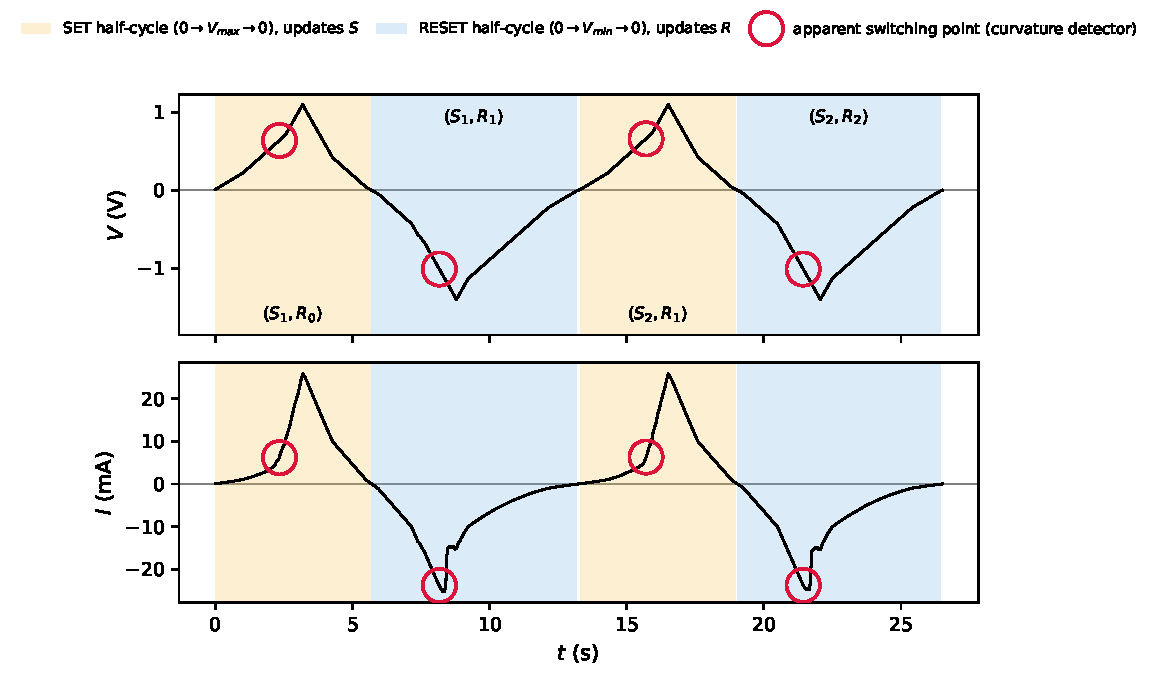
\includegraphics[width=\linewidth]{figures/fig_cycle_segments.pdf}
  \caption{Two real, consecutive full cycles (3000--3001): applied voltage
  (top) and measured current (bottom), with the four half-cycle spans
  shaded and labeled by the parameter pair the chain fit actually uses for
  that window, following Eq.~\eqref{eq:chain-sequence}. Only one side's
  index advances per half-cycle; the other side's value carries over
  unchanged from the previous window. The open circles are a loose,
  approximate marker of where each half-cycle's own apparent switching
  point sits, located by the same curvature-based detectors described in
  Section~\ref{sec:direct} ($d^2I/dt^2$ for SET, $d^3I/dt^3$-before-$d^2I/dt^2$
  for RESET) -- shown here to make visible, on real data, roughly where
  within each shaded span the transition driving that span's own parameter
  update actually happens, not as a precise measurement of $v_s$ or $v_r$.}
  \label{fig:cycle-segments}
\end{figure}

\section{Fitting procedure}
\label{sec:fitting}

\subsection{Production chain fit}

The dataset is a real measurement on a TiN/Ti/HfO$_2$/W device from the
same research group and measurement line as \cite{garcia2023temperature},
a sequence of triangular voltage sweeps, each cycle tracing
$0 \to V_{max} \to 0 \to V_{min} \to 0$. We split each cycle into its two
half-cycles -- $0 \to V_{max} \to 0$ (SET side active) and
$0 \to V_{min} \to 0$ (RESET side active) -- found from the raw voltage's
own zero crossings, with no detection logic beyond that. Each half-cycle is
fit independently by a joint, simultaneous least-squares call over its own
five (SET) or six (RESET) free parameters, with the other side's parameters
held fixed at their value from the immediately preceding half-cycle and the
internal state $g$ carried forward exactly (the ending $g$ of one half-cycle
becomes the starting $g$ of the next, never reset). The residual vector
includes both the current $I(t)$ and, by default, a smoothed $dI/dt$, since
matching the current alone without penalizing its derivative was found
early on to admit visibly wrong fits with an unremarkable aggregate error.

Three safeguards, each added after a specific documented failure mode,
make this procedure usable across the full dataset rather than a few
hundred cycles at a time:

\begin{itemize}
\item \textbf{A pin-escape margin.} Any of the twelve parameters that drifts
  within 5\% (in log space, for the log-scaled parameters) of its own global
  bound is reset to a geometric-mean value before the next half-cycle, to
  stop a parameter from ratcheting toward a bound and never returning.
\item \textbf{A capped $\eta_s, \eta_r$ range and a fixed $\gamma$.} Left
  free, $\gamma$ and $\eta_r$ trade off against each other: across roughly a
  threefold range of $\gamma$, a compensating $\eta_r$ reproduces the data to
  within 0.2--5.1\% error, a textbook flat ridge in the joint objective, not
  a sharp minimum. Fixing $\gamma = 0.22$ and capping
  $\eta_s, \eta_r \le 300$ removes this ridge; both choices are validated
  against the model's own cost surface, not asserted by convention.
\item \textbf{An rmse-spike retry.} A half-cycle whose fit error exceeds
  three times a rolling baseline (the median of the preceding 50 half-cycles)
  is refit once from a geometric-mean restart rather than from the possibly
  already-bad carried-forward value, keeping whichever attempt fits better.
  This catches a specific, otherwise fatal failure mode: a half-cycle whose
  own applied voltage range cannot physically reach its carried-forward
  $v_s$ or $v_r$ sits in an exactly flat region of the cost surface (we
  measured bit-for-bit identical residuals for $v_r$ perturbed by
  $\pm0.1\,$V around the stuck value), where a gradient-based optimizer has
  no local signal to climb out on and simply returns its starting point. A
  single such half-cycle, unpatched, derailed 69\% of a full 16\,602-cycle
  run and never recovered.
\end{itemize}

With all three in place, a full 14\,604-cycle run (cycles 2000--16603) gives
a SET-side peak-current error of 0.7\% (median) with only 0.09\% of
half-cycles exceeding 10\% error, and a RESET-side peak-current error of
1.7\% (median, 5.35\% of half-cycles above 10\%); the fit never freezes for
more than a handful of consecutive half-cycles anywhere in the run. Figure
\ref{fig:fit-overlay} shows one such window: the fit tracks the measured
current closely through the transition, with the largest local deviation
visible on the rising edge just before the peak, a reminder that ``low
aggregate rmse'' and ``correct everywhere'' are not the same statement.
Figure~\ref{fig:iv-loops} shows five consecutive raw measured cycles, to
give a sense of what this dataset's major loop and its cycle-to-cycle
repeatability actually look like before any fitting is applied.

\begin{figure}[t]
  \centering
  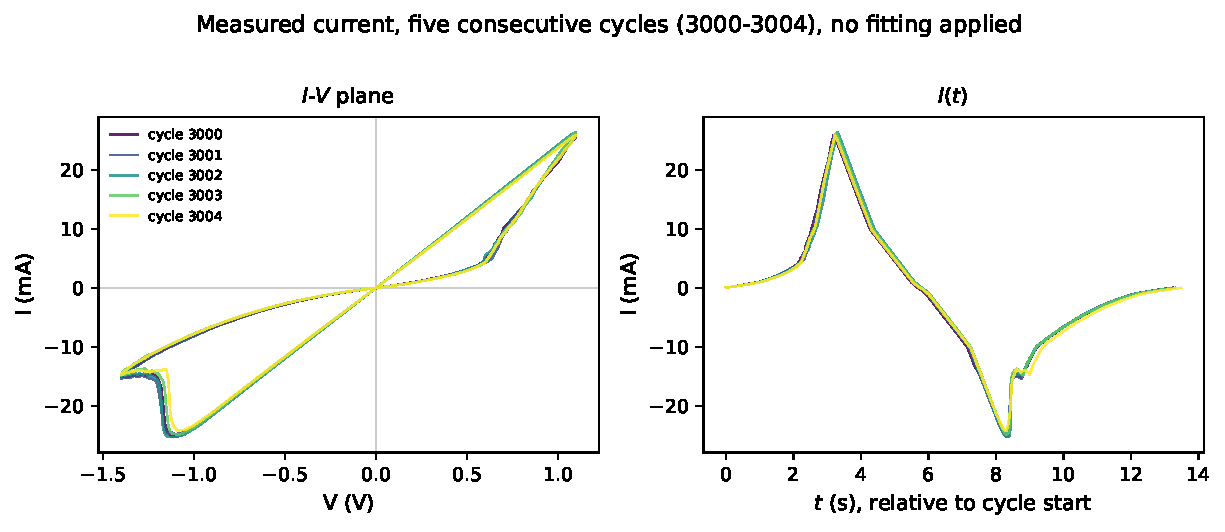
\includegraphics[width=\linewidth]{figures/fig1_iv_loops.pdf}
  \caption{Measured current, five consecutive raw cycles (3000--3004), no
  fitting applied. Left: the major $I$-$V$ hysteresis loop. Right: the same
  five cycles' current against time, relative to each cycle's own start.
  Both the loop shape and the time trace are stable from cycle to cycle,
  which is precisely what makes the waveform-diversity argument of
  Section~\ref{sec:difficulty} bite: every cycle probes essentially the
  same region of $(V,g)$ space, at essentially the same rate.}
  \label{fig:iv-loops}
\end{figure}

\begin{figure}[t]
  \centering
  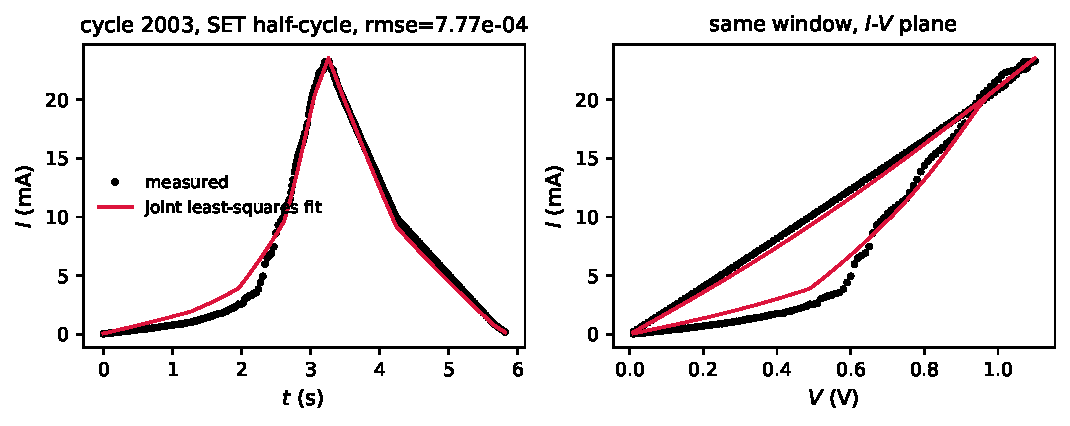
\includegraphics[width=\linewidth]{figures/fig2_fit_overlay.pdf}
  \caption{A real SET half-cycle window (cycle 2003) fit by the joint
  least-squares procedure. Left: measured and fitted current against time.
  Right: the same data in the $I$-$V$ plane. The fit is close but not
  exact; the largest local deviation sits on the rising edge, just before
  the current peak.}
  \label{fig:fit-overlay}
\end{figure}

\subsection{Five extraction strategies}

We compare five ways of solving each half-cycle's local optimization
problem, all sharing the chain-level procedure above:

\begin{description}
\item[lsq] \texttt{scipy.optimize.least\_squares} (trust-region-reflective),
  warm-started from the previous half-cycle's own fit. The fastest method
  tested (roughly 5--25 half-cycles/s depending on configuration) and, on
  both real data and the synthetic ground truth of
  Section~\ref{sec:montecarlo}, the most accurate on average.
\item[GA] \texttt{scipy.optimize.differential\_evolution}, with whichever of
  $v_s/v_r$ is this half-cycle's own free threshold locked to a narrow
  window around a direct, curvature-based estimate of that threshold
  (Section~\ref{sec:direct}), so the population search does not wander far
  from a value the data itself weakly constrains. Roughly 20--40 times
  slower than lsq.
\item[directed GA] Our own earlier method \cite{garciamoreno2008directed},
  reimplemented for this model: each generation, the residual Jacobian at
  the current best point is used to build the Gauss--Newton approximation
  $J^\top J$, whose eigendecomposition gives a local principal-axis frame;
  new individuals are Gaussian steps in that frame, with step size scaled by
  $\sqrt{\lambda_i/\lambda_{max}}$ so the stiffest directions are searched
  more aggressively, mixed with a 30\% isotropic-random fraction so the
  population cannot get trapped crawling a sloppy valley floor. Roughly 5.7
  times faster than plain GA at comparable fit error.
\item[GA+lsq] A multi-start hybrid: the full final population of a
  differential-evolution run, not just its best member, is individually
  polished by a bounded local least-squares step, and the best polished
  candidate is kept. The most expensive method tested, at roughly 17 times
  lsq's cost.
\item[CNN+lsq] A feed-forward network (not a true 1-D convolutional
  architecture in the run reported here, a limitation we return to in
  Section~\ref{sec:difficulty}) trained to map a half-cycle's resampled
  current and voltage traces, together with the fixed side's parameters and
  $g_0$, directly to the free side's parameters, trained on synthetic
  curves generated from realistic parameter combinations rather than a
  uniform prior over the box bounds -- a uniform prior was tried first and
  gave a training set dominated by curve shapes nothing like a real
  device's fit, which produced a catastrophic standalone evaluation. The
  network's output seeds one local least-squares polish before being
  reported.
\end{description}

\section{Extraction relations derived from the model's own equations}
\label{sec:direct}

Alongside the five optimization-based strategies above, the DMM's own
algebra yields several relations that can be checked exactly, in closed
form, against the model equations of Section~\ref{sec:model}, rather than
being validated only empirically. We derive the general result they all
specialize from, then list each one together with why it holds, since this
project also tried several plausible-looking shortcuts that turned out
\emph{not} to hold, and the distinction matters for anyone reusing this
methodology.

\subsection{General decomposition of $dI/dt$}
\label{sec:decomposition}

Write $K_a \equiv K(a_{on},a_{off},g)$, $K_i \equiv K(i_{on},i_{off},g)$,
$R_s \equiv K(r_{on},r_{off},g)$ for the three state-dependent blends of
Section~\ref{sec:model}, each affine in $g$ with slope $(a_{on}-a_{off})$,
$(i_{on}-i_{off})$, $(r_{on}-r_{off})$ respectively. From
$I(V_A,g) = K_i \sinh(K_a V_A)$, the two partial derivatives are
\begin{align}
J &\equiv \left.\frac{\partial I}{\partial V_A}\right|_g = K_i K_a \cosh(K_a V_A), \label{eq:J}\\
\left.\frac{\partial I}{\partial g}\right|_{V_A} &= (i_{on}-i_{off})\sinh(K_a V_A) + K_i V_A \cosh(K_a V_A)(a_{on}-a_{off}). \label{eq:dIdg}
\end{align}
Differentiating the series relation $V = V_A + R_s(g)\,I(V_A,g)$ with
respect to $t$ along a trajectory $(V_A(t), g(t))$ gives
\begin{equation}
\frac{dV}{dt} = \big(1 + R_s J\big)\frac{dV_A}{dt} + \underbrace{\Big[(r_{on}-r_{off})\,I + R_s \frac{\partial I}{\partial g}\Big]}_{\displaystyle C}\frac{dg}{dt},
\end{equation}
which rearranges to $dV_A/dt = \big(dV/dt - C\,dg/dt\big)/(1+R_s J)$. Substituting
into $dI/dt = J\,dV_A/dt + (\partial I/\partial g)\,dg/dt$ and collecting terms gives
the exact decomposition
\begin{equation}
\boxed{\;\frac{dI}{dt} = A(V,g)\,\frac{dV}{dt} + B(V,g)\,\frac{dg}{dt}\;},
\qquad
A \equiv \frac{J}{1+R_s J}, \qquad
B \equiv \frac{\partial I}{\partial g} - A\,C.
\label{eq:decomposition}
\end{equation}
This is exact, not a small-signal approximation; it is an identity given the
model's own equations, true at every sample of a trajectory the forward
model has already produced. Used that way, on a trajectory from
\texttt{dmm.simulate()}, it is a diagnostic: a way to check a candidate
fit's own internal consistency. Its use as an \emph{extraction} tool, on raw
data where $V_A(t)$ and $g(t)$ are not known, comes instead from three
special cases below where the slow term either vanishes or can be
cancelled, leaving only quantities measurable directly from $(t,V,I)$.

\paragraph{A diagnostic the decomposition gives for free: incomplete
switching at the turning point.} Apply Eq.~\eqref{eq:decomposition} on
each side of $V_{max}$ separately, normalizing by the ramp rate $r$ so the
sweep's own direction reversal ($dV/dt = +r$ before, $-r$ after) is
divided out and does not by itself masquerade as a slope change. SET's
hard gate means $dg/dt|_{t_0^-} = (1-g)S(V_A)$ immediately before the turn
and $dg/dt|_{t_0^+} = 0$ immediately after, so
\begin{equation}
\left.\frac{dI}{dV}\right|_{t_0^-} - \left.\frac{dI}{dV}\right|_{t_0^+}
= \frac{B\,(1-g)\,S(V_A)}{r}.
\label{eq:kink-asymmetry}
\end{equation}
\emph{This vanishes if and only if $(1-g)=0$.} In other words, a
measurable kink in the $I$-$V$ loop right at $V_{max}$ -- the pre-turn and
post-turn slopes visibly disagreeing, rather than the loop turning
smoothly -- is not a measurement artifact or a modeling inconvenience: it
is direct, exact evidence, from the model's own equations, that $g$ had
\emph{not} reached 1 by the time the sweep reversed, i.e.\ that SET was
still incomplete at $V_{max}$. Had the device fully saturated before the
sweep turned around, $(1-g)$ would already be zero on the pre-turn side as
well, Eq.~\eqref{eq:kink-asymmetry} would vanish, and the loop would turn
smoothly. The real loops in Figure~\ref{fig:iv-loops} and the fitted window
in Figure~\ref{fig:fit-overlay} both show a visible, non-smooth corner at
their own turning points, consistent with $g$ sitting strictly inside
$(0,1)$ there rather than at either extreme -- not a special or
occasional occurrence in this dataset, but the typical case. (The
symmetric argument at $V_{min}$ does not hold the same way, since RESET is
not sweep-direction gated and $dg/dt$ does not jump there; this diagnostic
is specific to the SET side's hard gate.)

We flag this as an \emph{added} difficulty for extraction, on top of the
parameter non-identifiability discussed in Section~\ref{sec:difficulty}:
it means the internal state cannot be treated, even approximately, as
``reset'' to a known boundary value (0 or 1) at either end of a sweep --
the state the device is actually in at any turning point is itself an
unknown, interior value, set by the full prior trajectory (how far
switching had already progressed when the previous half-cycle ended, how
much of the current half-cycle's finite duration was available for the
present transition to run, and the sweep's own rate). This is precisely
why the production chain fit of Section~\ref{sec:fitting} carries $g$
continuously across half-cycles, via \texttt{g0\_override}, rather than
resetting it: no cycle in this dataset can be fit correctly in isolation,
starting from an assumed fully-off or fully-on state, and the degree of
completeness at each turning point is one more quantity entangled with the
already weakly-identified rate parameters $\eta_s, \eta_r$ rather than a
simplifying boundary condition we can take for granted.

\subsection{Near-$V=0$ series resistance}

Deep inside a SET or RESET plateau, far from any transition, $g$ is
effectively frozen ($dg/dt \approx 0$) and $V_A \approx 0$. At $dg/dt=0$,
Eq.~\eqref{eq:decomposition} reduces to $dI/dt = A\,dV/dt$, i.e.\
$dI/dV = A$; evaluating $A$ at $V_A \approx 0$, where
$J = K_i K_a \cosh(0) = K_i K_a$ from Eq.~\eqref{eq:J}, gives
\begin{equation}
\left.\frac{dI}{dV}\right|_{V\approx 0} = A\big|_{V_A=0} = \frac{K_a K_i}{1 + R_s K_a K_i},
\qquad\text{equivalently}\qquad
\frac{1}{\text{slope}_0} = R_s + \frac{1}{K_a K_i},
\label{eq:nearzero}
\end{equation}
confirmed numerically exact against the forward model, and a direct
corollary of the general decomposition rather than a separate result. This
lets $R_s$ be solved in closed form given a measured near-zero slope and a
trial $(K_a, K_i)$ -- the basis of \texttt{derive\_ron}/\texttt{derive\_roff}
-- or, with no trial values at all, a crude but useful seed
$R_s \approx 0.5/\text{slope}_0$ (\texttt{estimate\_rs\_half}), motivated by
an independent check that this 50/50 split between the series resistance
and the fast element's own resistance holds on average across real SET
windows. The relation is provably exact on the ON side, which has a
genuine frozen-$g$ segment near $V=0$; it does not transfer to the OFF
side, which never fully freezes for $V<0$ in this model -- a real
identifiability limit of a single window's data, not an implementation
gap.

\subsection{Turning-point asymmetry}

At any sweep turning point, $dV/dt=0$ by definition, so
Eq.~\eqref{eq:decomposition} collapses to $dI/dt = B\,dg/dt$: the slow term
alone, exactly, with no approximation. What is \emph{not} symmetric is what
happens on either side of that point, because of the gating in
Section~\ref{sec:model}'s own $dg/dt$ equation: at $V_{min}$, RESET
kinetics ($dg/dt = -gR(V_A)$) are indifferent to sweep direction, so a
finite-difference estimate of $A$ built from samples on either side of the
turning point is unbiased either way. At $V_{max}$, SET kinetics switch off
\emph{exactly} at the peak ($H(dV/dt)$ is a hard gate, not a smooth one),
so $dg/dt$ jumps from $(1-g)S(V_A)$ to precisely zero the instant the sweep
turns, rather than merely changing sign. Immediately after the peak,
Eq.~\eqref{eq:decomposition} therefore reduces further, to
$dI/dt|_{t_0^+} = A\,dV/dt|_{t_0^+}$ with no slow-term contamination at
all -- a clean, single-sided read of $A$ -- while the pre-peak sample still
carries a live, nonzero $B\,dg/dt$ term that a symmetric two-sided
estimate would wrongly average in. The practical consequence, confirmed
against a synthetic ground truth over 600 real half-cycle windows: the
post-peak slope \emph{alone} gives a median $A$ error of 0.13\% at
$V_{max}$, while averaging in the pre-peak sample -- the natural thing to
do for a symmetric finite difference -- actively hurts (57\% median
error), exactly as the asymmetric gating above predicts. At $V_{min}$, by
contrast, all finite-difference variants agree to within a few percent,
exactly as the symmetric derivation predicts.

\subsection{Mid-sweep kinks}

\begin{figure}[h]
  \centering
  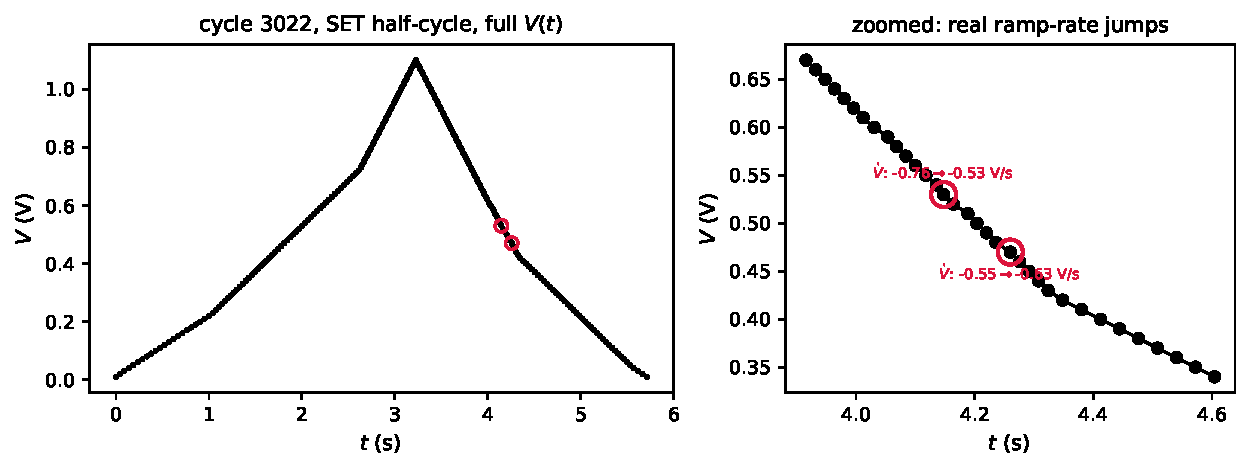
\includegraphics[width=\linewidth]{figures/fig_midsweep_kinks.pdf}
  \caption{The real applied-voltage sweep is not a constant-rate ramp.
  Left: one full real SET half-cycle's $V(t)$ (cycle 3022), with the
  ramp-rate changes visible as genuine corners, not smoothing artifacts.
  Right: a zoomed-in stretch of the same curve, with two ramp-rate jumps
  located by \texttt{find\_mid\_sweep\_kinks()} (same detector and
  default thresholds as the validation below), each labeled with its own
  measured $\dot V$ before and after.}
  \label{fig:midsweep}
\end{figure}

The real instrument does not ramp at a constant rate; it holds one
$dV/dt$ for a run of samples and then jumps to another, visibly so, as
Figure~\ref{fig:midsweep} shows directly on real data: the left panel is
one full real half-cycle's $V(t)$, with a piecewise-linear, not smoothly
curved, shape even at this scale; the right panel zooms into a short
stretch of it and marks two genuine ramp-rate jumps found by the same
detector described below, each with its own before/after $\dot V$.
Across such a jump,
if $g$'s own gate state does not change and $dg/dt$ is locally constant
(not zero, merely unchanging across the two samples), Eq.~\eqref{eq:decomposition}
gives, for the difference between the two sides of the jump,
\begin{equation}
\Delta\!\left(\frac{dI}{dt}\right) \approx A\,\Delta\!\left(\frac{dV}{dt}\right)
\quad\Longrightarrow\quad
A_{\text{apparent}} = \frac{\Delta(dI/dt)}{\Delta(dV/dt)},
\label{eq:midkink}
\end{equation}
the $B\,dg/dt$ term having cancelled in the difference rather than vanished
outright -- the same mechanism as the turning-point case, applied as a
two-point finite difference instead of a one-sided limit, and usable
anywhere in the sweep where the raw instrument happens to change its own
ramp rate, not only at $V_{max}/V_{min}$. We use two filters before trusting
a candidate jump: $dV/dt$ itself must be near-constant on \emph{both}
neighboring samples (rejecting multi-sample instrument transients that
would otherwise straddle a continuous ramp rather than two genuine
plateaus), and the jump must not sit too close to the window's own peak
voltage (checked per half-cycle piece, since a whole-cycle check
under-filters whichever side has the smaller peak magnitude). Validated
over 200+ real half-cycles against synthetic ground truth: median $A$ error
around 7\%, with the outliers explained almost entirely by $|dg/dt|$ itself
-- outlier kinks sit at a median $|dg/dt| \approx 0.42$, clean ones at
$\approx 1.2\times10^{-5}$ -- i.e.\ Eq.~\eqref{eq:midkink} fails
specifically where its own ``locally constant $dg/dt$'' assumption breaks
down, inside actively switching regions, not simply near a threshold
voltage. The companion slow-term read, $C_{\text{apparent}} = dI/dt|_k -
A_{\text{apparent}}\,dV/dt|_k$, is recoverable from the same pair wherever
$dg/dt$ is genuinely non-negligible (median 12\% relative error there), but
is a meaningless near-zero-denominator artifact in the roughly 75\% of
kinks that sit in an already-frozen-$g$ region.

\subsection{Curvature-based threshold estimators}

Unlike the three relations above, this one is motivated analytically but
not exact, and we are explicit about that distinction. Near a SET
transition, $I$ depends on $g$ only through the affine blends $K_a(g),
K_i(g)$, so by the chain rule $d^2I/dt^2$ picks up a term proportional to
$d^2g/dt^2$ on top of the purely fast ($dV_A/dt$-driven) contribution
already covered by Eq.~\eqref{eq:decomposition}. Since
$dg/dt = (1-g)S(V_A)$ with $S(V_A) = 2e^{-\eta_s v_s}\sinh(\eta_s V_A)$
growing rapidly once $V_A$ exceeds roughly $v_s$, $d^2g/dt^2$ itself peaks
near where the SET rate's own growth is fastest -- which is correlated with,
but not identical to, the crossing $V_A = v_s$, because the $(1-g)$ prefactor
and the fast-term contribution both shift the location of the maximum away
from $v_s$ by an amount that depends on the whole free-parameter side, not
on $v_s$ alone. This is why the resulting detectors below are usable
\emph{indicators} but not substitutes for $v_s, v_r$ themselves. Two such
detectors locate an
\emph{apparent} $v_s$ or $v_r$ directly from the curve's own shape: the
first positive peak of $d^2I/dt^2$ outside a margin around $V=0$ (excluding
a real but unrelated artifact from the instrument's own acquisition-rate
schedule), and the peak of $d^3I/dt^3$ at or before the peak of $d^2I/dt^2$,
which for $v_r$ specifically nearly doubles the correlation with the true
model value over the plain second-derivative detector (0.247 to 0.513 in a
synthetic check). Both derivatives are smoothed on a uniform \emph{time}
grid, not a fixed sample count -- real acquisition $dt$ varies several-fold
within a single window, and smoothing by sample count badly distorts a
second or third time derivative under that kind of jitter. We stress what
these detectors are \emph{not}: they correlate only weakly to moderately
with the true model $v_s, v_r$ (0.42--0.45 at best, uncalibrated), because
the apparent threshold they locate depends on the whole SET or RESET
nonlinearity, not on $v_s$ or $v_r$ in isolation. An earlier version of this
project used them as the \emph{reported} parameter value and as a hard
constraint fixed inside the joint optimizer; both uses failed outright (the
fixed-threshold variant produced unphysical fits in essentially every
window, since the internal voltage $V_A$ often cannot reach the apparent
threshold at all given realistic fast-side parameters). They are correct
and useful only as an input \emph{feature} alongside the raw curve, which
is how they are used in the CNN+lsq method of Section~\ref{sec:fitting}.

\subsection{A non-gradient alternative: the rule-based parameter extractor}
\label{sec:fuzzy}

Every method in Section~\ref{sec:fitting} is, underneath, a gradient
descent or a population search against a single joint cost function. The
tooling released alongside this paper (Appendix~\ref{app:tool}) also
includes a sixth, categorically different procedure: a rule-based
parameter extractor, labeled the \emph{fuzzy extractor} in the viewer's
own tab, the name it inherited from the version it evolved from. That
earlier version genuinely worked by $\pm1$-vote fuzzy-logic rules, one
per parameter, combined and thresholded each round; it proved hard to
calibrate and audit, and the mechanism described below is its
successor, keeping the one-rule-per-parameter spirit but replacing the
voting with the direct, per-parameter correction detailed next.

The current procedure never computes a joint Jacobian, a population, or
even a single joint cost value: \texttt{rmse} is simulated and recorded
purely as a reported diagnostic, by explicit design, and never decides
whether a step is accepted or when the procedure stops. Instead, each of
the ten free parameters ($\gamma$ held fixed, $g_0$ pinned by
continuity, as throughout this paper) has its own extraction procedure,
mapping a $(t,V,I)$ curve directly to a value in that parameter's own
physical units. Several of these are exactly the relations of
Section~\ref{sec:direct} applied literally, rather than used only as a
GA lock or a CNN input feature: $v_s, v_r$ from the curvature detectors
of Section~\ref{sec:direct}'s last subsection, $r_{on}, r_{off}$ from
the near-$V{=}0$ relation of
Eq.~\eqref{eq:nearzero}. One relation appears here for the first time:
$\eta_s, \eta_r$ are read from the full width at half maximum, in time,
of smoothed $|dI/dt|$'s own peak at the transition -- a narrower peak
means faster switching, i.e.\ a larger $\eta_s$ or $\eta_r$, a direct
geometric reading rather than a fit.

At each visit, the parameter's own procedure is applied once to the
real data and once to the model's own current simulated curve over the
same window; the correction is driven by the difference between the two
-- additive, directly in volts, for $v_s, v_r$; multiplicative, in log
space, for the rest -- a genuine Newton-style correction in the
parameter's own physical units, not a step along a joint gradient and
not a vote. Parameters are visited one at a time, in a fixed order
($v_r, v_s, i_{on}, r_{on}, r_{off}, a_{on}, a_{off}, i_{off}, \eta_s,
\eta_r$), one correction per visit, for repeated full passes (up to 40)
until a pass moves nothing. A real divergence found during development
motivated capping each individual correction (to $\pm2\%$): an
undamped multiplicative step could swing $i_{off}$ by a factor of 50 in
one update, which then corrupted $r_{off}$'s own near-$V{=}0$
extraction in turn (Eq.~\eqref{eq:nearzero} reads $r_{off}$ off a
measurement that itself depends on $i_{off}$) -- a small, self-contained
instance of exactly the kind of parameter entanglement
Section~\ref{sec:difficulty} documents at the whole-chain scale.

We report this method's mechanism and design rationale in detail because
of its interpretability -- every update is a one-line, physically
readable statement (\emph{``the data's transition is narrower than the
model's own, so raise $\eta_s$''}), auditable without any
optimization-theory background, which none of the five methods in
Section~\ref{sec:fitting} offer. We also ran it through the same
500-half-cycle Monte Carlo ground-truth benchmark as those five
(Section~\ref{sec:montecarlo}); the result is not a quantitative win --
it is, if anything, the single clearest illustration in this paper of
why the problem is hard, discussed alongside the other five methods'
own results there rather than separately here.

\section{Monte Carlo ground-truth comparison}
\label{sec:montecarlo}

Comparing extracted parameters against each other, or against previous runs
of the same method, cannot distinguish ``converged to the correct answer''
from ``converged to the same wrong answer as last time.'' We instead built
a test with a known, exact ground truth: 500 half-cycles (250 full cycles)
of parameters, taken directly from a real chained GA fit, were used to
forward-simulate noise-free synthetic current over each half-cycle's own
real $(t,V)$ excitation. Every extraction strategy was then re-run on this
synthetic data, blind to the generating parameters, and the recovered
values compared against the known truth.

\begin{table}[t]
\centering
\small
\caption{Correlation between extracted and true parameter values, 500-half-cycle
noise-free Monte Carlo test. Bold marks the best method per row. ``n/a''
(rule-based column) means the refit value never changed from its initial
seed across the entire 250-cycle run -- not a weak correlation, zero
variation to correlate against at all; counted as 0 in that column's
average.}
\label{tab:montecarlo}
\begin{tabular}{lrrrrrr}
\toprule
parameter & lsq & GA & directed GA & GA+lsq & CNN+lsq & rule-based \\
\midrule
$v_s$     & \textbf{0.31} & 0.18 & 0.14 & 0.16 & 0.21 & $-$0.16 \\
$\eta_s$  & 0.65 & 0.60 & 0.72 & \textbf{0.89} & 0.04 & $-$0.03 \\
$r_{on}$  & 0.64 & \textbf{0.79} & 0.72 & 0.78 & 0.48 & n/a \\
$a_{on}$  & \textbf{0.45} & 0.21 & 0.30 & 0.27 & 0.35 & n/a \\
$i_{on}$  & 0.24 & 0.06 & 0.00 & 0.04 & \textbf{0.78} & n/a \\
$v_r$     & 0.54 & 0.45 & 0.39 & 0.45 & \textbf{0.70} & $-$0.15 \\
$\eta_r$  & \textbf{0.63} & 0.13 & 0.18 & 0.07 & 0.18 & $-$0.30 \\
$r_{off}$ & 0.27 & 0.28 & \textbf{0.47} & 0.41 & 0.10 & 0.08 \\
$a_{off}$ & \textbf{0.79} & 0.57 & 0.56 & 0.54 & 0.33 & n/a \\
$i_{off}$ & 0.44 & 0.57 & 0.44 & \textbf{0.64} & $-$0.07 & n/a \\
\midrule
average   & \textbf{0.50} & 0.38 & 0.39 & 0.42 & 0.31 & $-$0.06 \\
\bottomrule
\end{tabular}
\end{table}

Table~\ref{tab:montecarlo} and Figure~\ref{fig:method-comparison} give the
full result; Figure~\ref{fig:identifiability-scatter} shows the underlying
scatter for lsq on four representative parameters. Five findings stand out.

First, plain lsq has the best \emph{average} correlation of the six
methods (0.50), despite being by far the cheapest. Population-based and
hybrid methods do not buy accuracy here; GA+lsq, at roughly 17 times lsq's
cost, trails it by 0.08 on average. We take this as evidence that the
difficulty is not local-optimum trapping, which population methods are
designed to escape, but something that survives a global search as well.

Second, no method reaches even moderate correlation on $i_{on}$ except
CNN+lsq (0.78 against a next-best of 0.24), and no method does well on
$v_s$ (0.14--0.31 across the board). These two are the project's most
persistently non-identifiable parameters, and we return to why in
Section~\ref{sec:difficulty}.

Third, the CNN surrogate's error profile is qualitatively different from
every optimizer-based method, not merely worse or better: it is the best
method on $i_{on}$ and $v_r$ by a wide margin, and the worst on $\eta_s$,
$a_{off}$, $i_{off}$, dragging its average below every other method. A
network trained on realistic parameter \emph{combinations}, rather than
searching the current window in isolation, appears to encode a learned
prior over where real devices actually sit along the $(r_{on},a_{on},i_{on})$
ridge described in Section~\ref{sec:difficulty} -- information no local or
population search run on a single curve has access to, but exactly the kind
of information a single, fixed excitation waveform cannot by itself supply
(Section~\ref{sec:difficulty}). This was a single run of a flat,
fully-connected network with one random seed and no architecture search;
whether a properly convolutional, larger, ensembled version closes the gap
on the remaining parameters without losing the $i_{on}$/$v_r$ gain is, at
the time of writing, still an open, partially negative experiment (one
round of scaling up moved $v_r$'s correlation to roughly 0.52 under
teacher-forcing, but did not establish a clean win end to end).

Fourth, comparing this table against the same methods' agreement with each
other on \emph{real} (noisy) data is itself informative: lsq and GA agree
with each other on real data at correlations of only 0.01--0.26 across the
twelve parameters, far below what Table~\ref{tab:montecarlo} shows on
noise-free synthetic data (0.06--0.79). Most of that gap is explained by
real measurement noise destabilizing an already only weakly constrained
fit, not by a disagreement between the methods' underlying cost surfaces --
but the gap does not close to zero even with noise removed, which is the
residual, genuine non-identifiability this paper is about.

Fifth, the rule-based extractor of Section~\ref{sec:fuzzy} is the clearest
illustration of this paper's whole argument, not an outlier to it. A cold
start from the NOMINAL card never produces a single parameter update at
all on this data: the trial curve never switches enough to clear the
procedure's own switching-state gate, so every one of the ten free
parameters is skipped on the very first attempt. Chaining it cycle to
cycle instead -- bootstrapping the first cycle, then warm-starting every
subsequent one from the previous cycle's own output, the same continuity
argument Section~\ref{sec:model} makes for the other five methods --
avoids that complete stall, but on this blind, 250-cycle run five of
its ten free parameters ($r_{on}, a_{on}, i_{on}, a_{off}, i_{off}$)
never move even once past their very first bootstrap value, for the
\emph{entire} run; the other five move but correlate weakly or
negatively with truth ($-0.30$ to $0.08$). This is a sharper version of
the bound-pinning pattern Section~\ref{sec:difficulty} documents for
lsq/GA's $a_{on}$ (Figure~\ref{fig:bound-pinning}): there, an optimizer
still revisits the parameter every window and rides a flat direction to
a box edge; here, the gate that is supposed to protect each per-parameter
update from an untrustworthy trial curve ends up protecting a stale
value from ever being questioned again. We see this as independent
confirmation, by a method with no gradient, no population, and no
learned prior at all, that the difficulty documented throughout this
paper is a property of the data, not an artifact of any one optimization
strategy.

\begin{figure}[t]
  \centering
  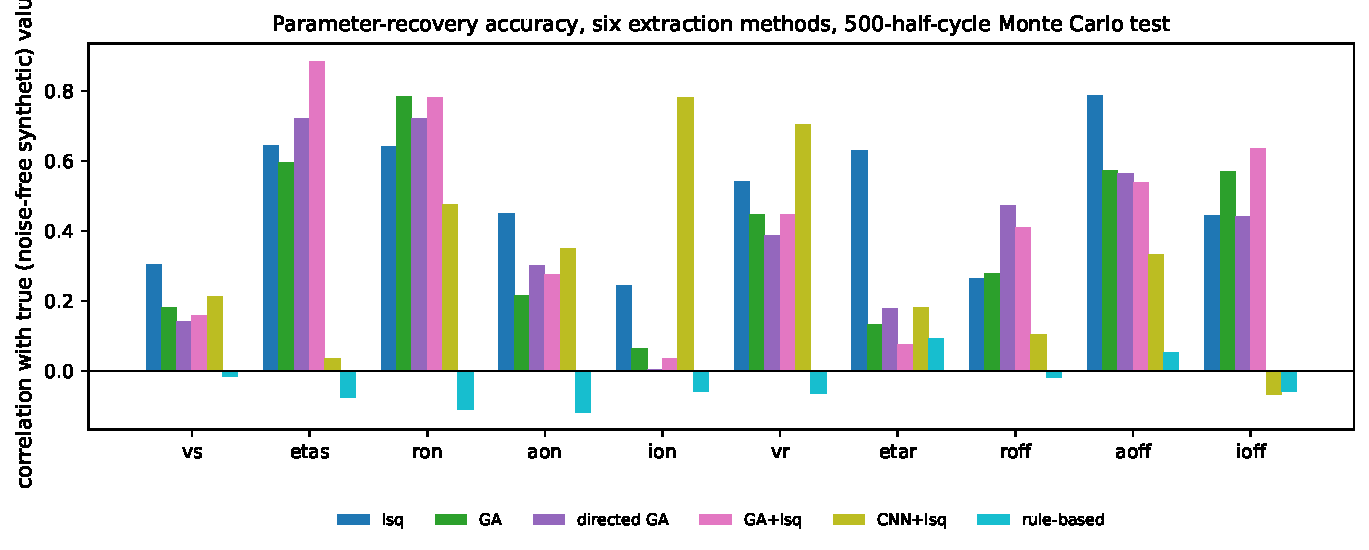
\includegraphics[width=\linewidth]{figures/fig5_method_comparison.pdf}
  \caption{Correlation with the true, noise-free synthetic parameter value,
  all ten free parameters, six extraction methods. No method is uniformly
  best; $i_{on}$ and $v_s$ are weakly recovered by every method except, for
  $i_{on}$, the CNN surrogate. The rule-based extractor's bars sit at 0 for
  $r_{on}, a_{on}, i_{on}, a_{off}, i_{off}$ because its own refit value
  never changed across the entire run on those five parameters -- zero
  variation to correlate against, not a weak correlation.}
  \label{fig:method-comparison}
\end{figure}

\begin{figure}[t]
  \centering
  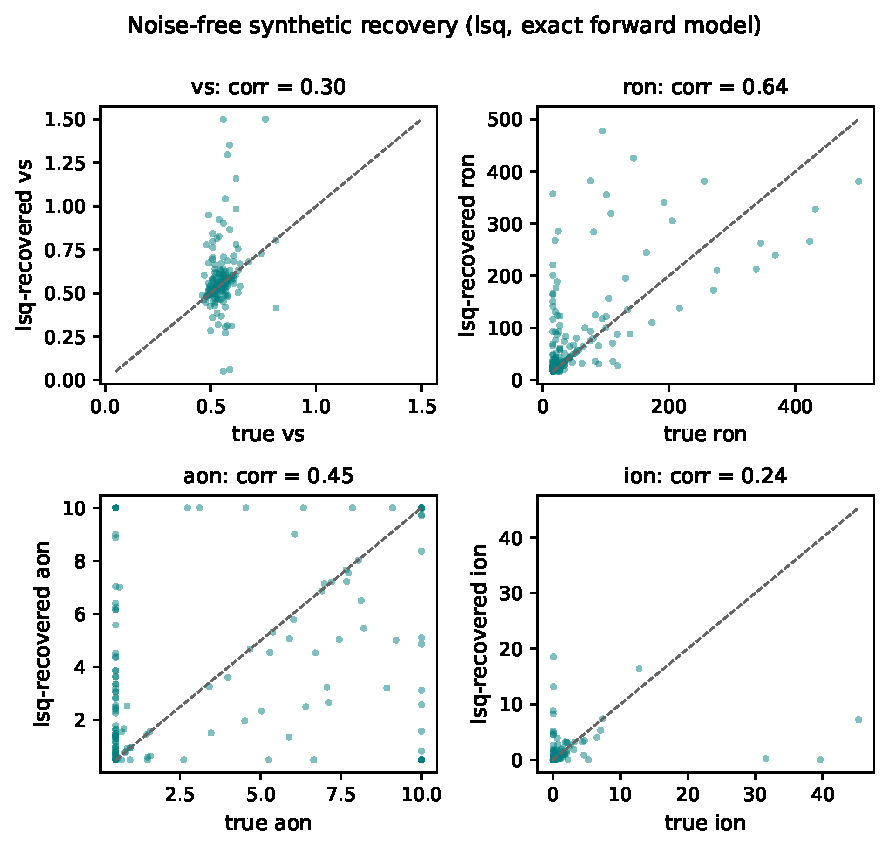
\includegraphics[width=0.78\linewidth]{figures/fig4_identifiability_scatter.pdf}
  \caption{True vs.\ lsq-recovered value, noise-free synthetic data, four
  representative SET-side parameters. $r_{on}$ clusters reasonably around
  the identity line; $a_{on}$ and $i_{on}$ do not.}
  \label{fig:identifiability-scatter}
\end{figure}

\section{Why fitting this model is hard}
\label{sec:difficulty}

The Monte Carlo test isolates the problem from measurement noise; it does
not yet explain it. We checked four candidate explanations directly,
rather than assume any of them.

\paragraph{A single, repeated excitation waveform.} Across the entire
usable dataset (cycles 2 through 16603), $V_{max}=1.100\,$V,
$V_{min}=-1.400\,$V, and the sample count per cycle are exactly identical,
with zero variance, cycle after cycle -- confirmed directly, not assumed.
There is no hidden amplitude sweep or rate variation anywhere in the
dataset to exploit. By the identifiability arguments of Chis and
Balsa-Canto \cite{chis2014sloppy} and White et al.\
\cite{white2016limitations}, a single fixed excitation, repeated, cannot
in general carry enough independent information to uniquely constrain
every parameter of a ten-to-twelve-parameter nonlinear ODE, regardless of
how the inverse problem is solved. We consider this the deepest root cause
of the pattern in Table~\ref{tab:montecarlo}: the specific parameters that
go unrecovered are consistent across all five methods, which is what this
explanation predicts and an optimizer-quality explanation does not.

\paragraph{The $\gamma$/$\eta_r$ ridge.} Already described in
Section~\ref{sec:fitting} as a fitting-procedure fix: RESET's rate depends
on $\eta_r\, g^{\gamma}$, and within a single half-cycle $g$ does not range
far enough for $\gamma$ and $\eta_r$ to be told apart. This is a genuine
algebraic near-degeneracy, confirmed by scanning $\gamma$ with $\eta_r$
re-optimized at each point and finding the data matched to within a few
percent across roughly a threefold range of $\gamma$. It is specific to the
model's own $g^\gamma$ term, and it is fully addressed by holding
$\gamma$ fixed; it is not the explanation for the remaining parameters.

\paragraph{Bound pinning on $a_{on}$.} Figure~\ref{fig:bound-pinning}
shows the distribution of $a_{on}$ across the Monte Carlo ground-truth set
(itself sourced from real GA-chain fits): 64\% of values sit at the lower
box bound, 14\% at the upper one. An optimizer pinned against a box
constraint, rather than converging to an interior optimum, is close to the
textbook signature of a flat direction in the cost function -- the search
rides it to the edge of the box and stops there for lack of anything to
distinguish points along it. A direct check of why: within real windows,
the product $K_a V_A$ -- the argument of the model's $\sinh$ nonlinearity
-- sits at a median of 0.3--0.8 and occasionally exceeds 2, which is too
large for the small-signal linearization $\sinh(x)\approx x$ to hold
cleanly across the whole window, yet the data still does not pin $a_{on}$
down on its own. We read this as consistent with, not contradicting, the
waveform-diversity explanation above: the window explores enough of the
nonlinearity to be sensitive to \emph{some} combination of $a_{on}$ and
$i_{on}$, but not enough, under one fixed excitation, to separate the two.

\begin{figure}[t]
  \centering
  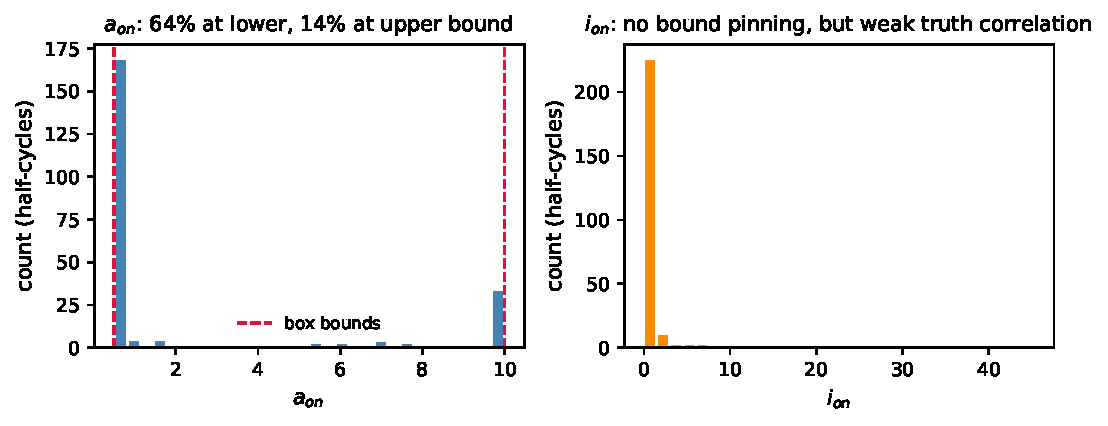
\includegraphics[width=\linewidth]{figures/fig3_bound_pinning.pdf}
  \caption{Distribution of $a_{on}$ and $i_{on}$ across the Monte Carlo
  ground-truth set (itself sourced from real fits). $a_{on}$ shows the
  classic bimodal pile-up at its own box bounds that a flat-direction
  optimizer produces; $i_{on}$ shows no such pile-up, yet is still poorly
  recovered (Table~\ref{tab:montecarlo}), which is why we tested the pooled
  hypothesis below rather than stopping at this figure.}
  \label{fig:bound-pinning}
\end{figure}

\paragraph{A pooled-fitting test, reported here for the first time.} The
most natural fix to try, given the bound-pinning result, is to ask whether
$a_{on}$ and $i_{on}$ are in fact device-level material constants that
should not vary from cycle to cycle at all, with the apparent per-window
scatter in Table~\ref{tab:montecarlo} and Figure~\ref{fig:bound-pinning}
being an artifact of fitting them independently under a weak per-window
constraint. We tested this directly on twelve real SET half-cycle windows,
spread across cycles 3000--8500 of the actual measured data (not synthetic),
comparing two fits: each window's own fully free 11-parameter fit, against
one joint least-squares problem over all twelve windows simultaneously,
with $a_{on}$ and $i_{on}$ forced to a single shared value and every other
parameter still free per window. If the hypothesis were correct, the pooled
fit should cost little.

It does not. The pooled fit is worse than the free fit by a factor of 14.6
on average, and -- this is the part that rules the hypothesis out rather
than merely weakening it -- \emph{uniformly} worse across all twelve
windows (Figure~\ref{fig:pooled-vs-free}), not concentrated in a few
outliers. The per-window free-fit values of $a_{on}$ and $i_{on}$ span a
wide range (0.50--8.7 and 0.098--15.4 respectively) that a shared constant
cannot absorb by adjusting the other nine free parameters per window; no
other parameter can compensate for a wrong nonlinearity shape. $a_{on}$ and
$i_{on}$ are therefore not simply masked constants: whatever each window's
best-fit value actually reflects, it moves window to window in a way a
single global value cannot capture, even though, per Section~\ref{sec:direct}
and the single-window flat-direction evidence above, it is also only weakly
determined \emph{within} any one window. The most consistent reading of
both results together is that this is a genuinely sloppy model in Chis and
Balsa-Canto's sense: a real, nearly flat direction exists in each window's
own cost surface, but its location shifts with the other, genuinely
cycle-varying parameters (plausibly real device drift in $r_{on}$, $v_s$,
or the switching rate), so no fixed point along it is right for every
window.

\begin{figure}[t]
  \centering
  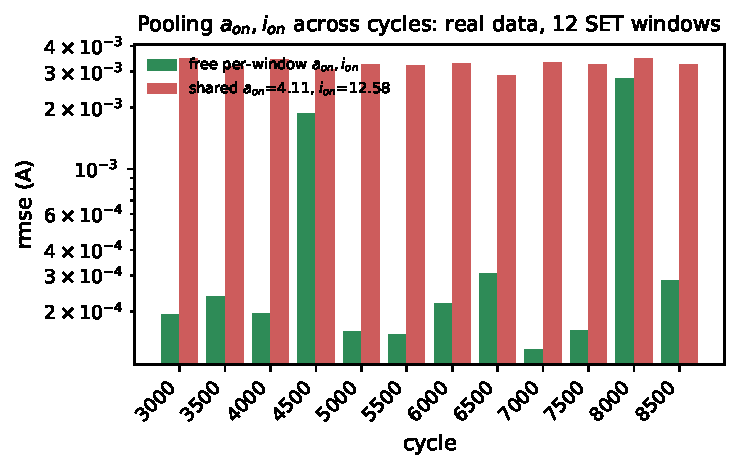
\includegraphics[width=0.85\linewidth]{figures/fig6_pooled_vs_free.pdf}
  \caption{Fit rmse, real data, twelve SET half-cycle windows (cycles
  3000--8500): each window fit fully independently, against one joint fit
  sharing a single $a_{on}, i_{on}$ pair across all twelve windows. The
  pooled fit is worse in every single window, not just on average,
  ruling out ``shared device constant hidden by noise'' as an
  explanation.}
  \label{fig:pooled-vs-free}
\end{figure}

Put together, these four checks point to the same conclusion from different
directions: the DMM's own equations are not over-parameterized in a way
that a cleverer reparameterization could fix for free (the one genuine
algebraic redundancy we found, $\gamma$ against $\eta_r$, is already
accounted for), and the remaining weak identifiability of $v_s$, $a_{on}$,
$i_{on}$, $\eta_r$ is a property of this specific, fixed-waveform dataset
interacting with a twelve-parameter nonlinear ODE, not a property any of
the five optimization strategies we tried could have fixed by searching
harder or more cleverly.

\section{Conclusions}
\label{sec:conclusions}

The DMM reproduces this dataset's measured switching current accurately: a
median peak-current error of 0.7\% on the SET side and 1.7\% on the RESET
side, across a 14\,604-cycle production chain fit, with no catastrophic
derailment once the $\gamma$/$\eta_r$ ridge and the window-reachability
failure mode of Section~\ref{sec:fitting} are addressed. Accurate current
reproduction and accurate parameter recovery are not the same claim,
however, and our central result is that they diverge substantially for a
specific subset of this model's twelve parameters -- most persistently
$v_s$, $a_{on}$, $i_{on}$, and $\eta_r$ -- across every one of five
genuinely different extraction strategies, spanning gradient descent,
population search, a hybrid of the two, a method built explicitly around
the local Jacobian's principal directions, and a learned surrogate trained
on realistic synthetic data.

We do not think this reflects badly on the DMM specifically. The same
pattern -- parameters described in the literature as ``fitting parameters
without direct physical meaning,'' or reported saturating at search-space
bounds during a recent independent CNN-based extraction effort on a
different model entirely \cite{hamid2025cnn} -- recurs across essentially
every ReRAM compact model whose extraction procedure is documented in
enough detail to check. What this dataset adds, beyond the general
argument, is a direct, falsifiable demonstration that the obvious fix --
treat the weakly-identified parameters as shared constants across cycles --
does not work here, tested rather than assumed.

Two practical consequences follow. First, any downstream use of this
project's per-cycle parameter trajectories -- aging or degradation
analysis, for instance, which depends on treating cycle-to-cycle parameter
\emph{drift} as a physical signal -- should not be taken at face value for
$v_s$, $a_{on}$, $i_{on}$, or $\eta_r$ without independent corroboration;
the trajectory shape for these may reflect which point along a flat
direction the optimizer happened to land on, not a real physical change.
$r_{on}$, $a_{off}$, and (for GA-family methods) $\eta_s$ are recovered
considerably better and are safer to trust for this purpose. Second, since
the root cause we identify is a property of the experiment, not the
optimizer, the only extraction-side remedy left is an experimental one:
varying the sweep amplitude or rate across a subset of cycles, specifically
to give the fitting procedure information this dataset's single repeated
waveform structurally cannot supply. We have not attempted this, since it
requires new measurements rather than new analysis, but it follows directly
from the argument above and we would recommend it as the next step for
anyone extending this work.

\appendix
\section{The rolling-parameter analyzer}
\label{app:tool}

Every per-cycle figure in this paper (Figures~\ref{fig:fit-overlay},
\ref{fig:bound-pinning}, and the trajectory view used while diagnosing the
pin-escape and rmse-spike failure modes of Section~\ref{sec:fitting}) was
produced with the aid of a tool we release alongside this paper,
\cite{rollinganalyzer}:

\begin{center}
\url{https://github.com/rpicos-uib/rolling-parameter-analyzer}
\end{center}

It is a Tkinter desktop viewer over a chained-fit CSV (one row per
half-cycle, the twelve DMM parameters plus fit \texttt{rmse}), built
incrementally over the course of this project specifically because
aggregate statistics repeatedly hid real problems that only a direct,
per-cycle visual check caught -- the chain-damping, curve-inspector, and
window-reachability issues of Section~\ref{sec:fitting} were all found
this way, not from a summary number. It reads its input CSV on demand, so
it doubles as a live monitor for a still-running extraction job, and
provides six views:

\begin{figure}[h]
  \centering
  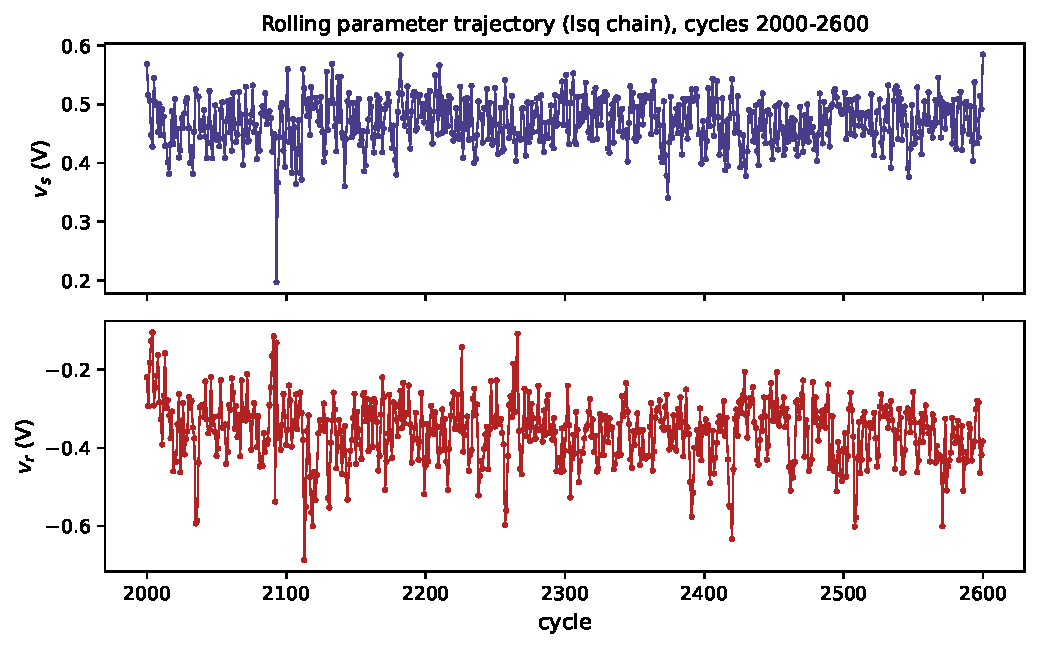
\includegraphics[width=0.85\linewidth]{figures/fig7_rolling_trajectory.pdf}
  \caption{The kind of trajectory the ``Evolution vs.\ cycle'' view is
  built to show: $v_s$ and $v_r$ as extracted by the production lsq chain,
  cycles 2000--2600. Consistent with the identifiability findings of
  Section~\ref{sec:difficulty}, this trajectory should be read as a
  noisy, only weakly constrained signal rather than a precise physical
  record of cycle-to-cycle drift.}
  \label{fig:rolling-trajectory}
\end{figure}

\begin{enumerate}
\item \textbf{Evolution vs.\ cycle} -- any subset of the twelve parameters,
  plus \texttt{rmse}, each independently rescaled to $[-1,1]$ so
  parameters on very different scales (e.g.\ $i_{off}\sim10^{-4}$ against
  $r_{on}\sim50$) can be read off one shared axis against cycle number. A
  cycle slider opens a popup overlaying the real measured curve against the
  model's own forward simulation, for the selected cycle and its
  neighbors, each with its own fitted parameters.
\item \textbf{Parameter vs.\ parameter} -- a scatter of any two parameters,
  same cycle or lagged by one, with a regression line and its $R^2$.
\item \textbf{Distribution} -- a histogram of one parameter (or
  \texttt{rmse}) with any combination of Gaussian, Lognormal, Gamma,
  Exponential, Logistic, Skew-normal, or Weibull fits overlaid, plain or as
  a $k$-component mixture.
\item \textbf{Parameter table} -- a live, scrollable table of all twelve
  parameters against cycles, centered on a chosen cycle.
\item \textbf{Curve inspector} -- actual-vs-model current and $I$-$V$ for a
  chosen cycle. This view required a specific fix during this project: a
  chain-fitted cycle has two different parameter sets in play, one before
  and one after its own RESET-side update, and a single merged simulation
  call across the whole cycle silently applies the wrong, later set to the
  earlier portion of the curve -- confirmed directly as the cause of a
  20--30\% spurious reconstruction error that had nothing to do with the
  underlying extraction, which was correct throughout.
\item \textbf{Fuzzy extractor} -- runs the project's interpretable,
  per-parameter iterative extraction procedure (Section~\ref{sec:fuzzy})
  live on one chosen cycle, showing each individual parameter update
  (which parameter, its own data-vs-model error, old and new value)
  rather than only a converged endpoint, as an alternative, steppable
  lens alongside the joint least-squares fit.
\end{enumerate}

Beyond the viewer itself, the repository also includes the fitting CLI
behind Section~\ref{sec:fitting} (\texttt{fit\_chain\_cli.py}, exposing
four of the paper's five extraction methods -- lsq, GA, directed GA, and
GA+lsq -- through one documented \texttt{--help}) and the Monte Carlo
ground-truth generator and comparison script behind
Section~\ref{sec:montecarlo} (\texttt{mc\_param\_recovery.py},
\texttt{compare\_vs\_truth.py}), all under the MIT license. A small
synthetic demo dataset is committed alongside them so every command the
repository's own README documents -- generate, fit, validate, inspect --
runs end to end on a fresh clone, with no dependency on the real
measurement data \cite{garcia2023temperature}, which is not included. The
paper's fifth method (the CNN surrogate) was a single exploratory pass,
as Sections~\ref{sec:fitting} and~\ref{sec:montecarlo} already note, and
its research-stage code is likewise not part of this release.

\bibliographystyle{IEEEtran}
\bibliography{references}

\end{document}
